\chapter{Selection Bias Removal}
This chapter 
is based on Ref.\cite{bare-sb-removal}.

Selection bias (SB)
occurs when one 
samples from an
atypical subset
of a
population,
producing a biased dataset.
Are such biased 
datasets
useless? Not necessarily. 
It is possible to 
add additional auxiliary features
to the biased dataset, and to 
sample those new features
in an unbiased way,
 from the whole population.
Then
one can merge
the original
 biased dataset with the
auxiliary, unbiased one,
to obtain an enhanced dataset.
It is sometimes
possible to do this so that the enhanced
dataset is provably 
unbiased.
It's like making horizontal
the surface of a table
 that was
 not initially
horizontal.
The theory of Bayesian Networks and Causal
Inference tells us 
WHEN this is possible,
and HOW to do it
when it is possible.

Consider the bnet 
Fig.\ref{fig-bs-removal-basic}.

\begin{figure}[h!]
$$
\xymatrix{
\rvs=1\ar[dr]|?\ar[d]_?\ar[r]^?
&\rvA\ar[d]
&
\\
\rvx\ar[r]\ar@/_.9pc/[ru]
&\rvy
}
$$
\caption{Bnet considered for 
selection bias (SB) removal.
Arrows with question marks
may or may not be present.}
\label{fig-bs-removal-basic}
\end{figure}

Let

$\rvs\in\bool$
is the {\bf selection node}.
$\rvs=1$ means there is 
SB
in the node.
$\rvs=0$ or no $\rvs$ parent
means there 
is no SB in the node.


$\rvx=$ {\bf class features}.\footnote{
A feature is the same as a node in a bnet.}

$\rvy=$ {\bf target feature}.

$\rvA=$ {\bf auxiliary features}
(Ref.\cite{bare-sb-removal} 
calls this $T-\{\rvx\}$) 

$\rvE=\{\rvy, \rvx\}\cup\rvA=$ 
{\bf Enhanced feature set}
(Ref.\cite{bare-sb-removal} calls this $M$) 

$\Sigma=$ population of individuals $\s$

$OD=\{(\s,\rvx^\s,  \rvy^\s,\rvs^\s=1):\s\in\Sigma\}=$ 
{\bf Original Dataset}, dataset for $(\rvx,\rvy)$ features
with $\rvs=1$. 
Gives empirical
distribution $\color{red}{P(y|x, \rvs=1)}$.
(Ref.\cite{bare-sb-removal} 
calls this dataset the {\bf biased study}.)

$AD=\{(\s, \rvx^\s,\rvA^\s):\s\in\Sigma\}=$ 
{\bf Auxiliary Dataset}, dataset for $(\rvx, \rvA)$ features.
Gives empirical
distribution $\color{red}{P(A|x)}$.
(Ref.\cite{bare-sb-removal} 
calls this dataset the 
{\bf population level study}.)


$ED=\{(\s,\rvx^\s, \rvA^\s, \rvy^\s,\rvs^\s=1):\s\in\Sigma\}=$ 
{\bf Enhanced Dataset}, dataset for $(\rvx,\rvy, \rvA)$ features
for $\rvs=1$.
Obtained by merging $OD$ and $AD$.
Gives empirical
distribution $\color{red}{P(y|x, A, \rvs=1)}$.

\section{Selection Nodes
and Selection Bias}
Selection
nodes can be a source
of confusion,
so it's worth 
spending some time
thinking about them.


Suppose that the nodes
of a bnet can be either
blue or colorless.
Then we can define 
a selection
node $\rvs_{blue}$
such that 
$\rvs_{blue}=1$
points
to the nodes that 
are blue, and
nothing
points
to the nodes that are 
colorless.
If we were to
change the value of 
node $\rvs_{blue}$ to
zero, 
then all the nodes 
of the bnet would be colorless.
Suppose instead that 
the nodes of a bnet
could be either
blue, red or colorless.
Then one could define 
two selection nodes,
$\rvs_{blue}$
and $\rvs_{red}$,
and 
draw arrows
from $\rvs_{blue}=1$
to the blue nodes
and from
$\rvs_{red}=1$
to the red nodes, and no arrow 
directed into the colorless nodes.
So, basically, selection nodes
are binary root nodes
that indicate 
whether the nodes pointed to
belong to a set or not.



In this chapter,
selection nodes
$\rvs\in\bool$
are {\color{red}root} nodes
whereas in
the paper Ref.\cite{bare-sb-removal}
on which this chapter
is based,
selection nodes $\rvs\in \bool$
are {\color{red}leaf} nodes.
Why the difference, and
are these two conventions
 equivalent, and if
they are, how does 
one translate
from one convention
to the other?


Suppose that we start with
a bnet $G_0$ that is fully connected, and 
we add to it a selection node $\rvs$ 
that is a root node that points
to all nodes of $G_0$.
Call the resulting bnet $\rvs\rarrow G_0$.
We can use Bayes rule to reverse the direction
of the arrows emanating from $\rvs$
so that they enter node $\rvs$ 
rather than exit
it.
Call the resulting bnet $\rvs\larrow G_0$.
In general,
Bayes rule allows us to translate 
from $\rvs\rarrow G_0$ to 
$\rvs\larrow G_0$,
or in the opposite direction,
without having to change the 
directions of any of the arrows in $G_0$.
If $G_0$ is not fully connected, then
going from
$\rvs\rarrow G_0$ to 
$\rvs\larrow G_0'$ 
will often require that $G_0'$
have the same arrows in the same
directions as $G_0$
plus some extra arrows
new to $G_0$.
Likewise, going
from
$\rvs\larrow G_0$ to 
$\rvs\rarrow G_0''$
may require that $G_0''$ have
the same arrows as $G_0$ plus some new arrows.
Recall that in Chapter \nameref{ch-bnet-def},
we made a distinction
between causally correct (CC)
bnets, and non CC bnets, and
we pointed out
that non CC bnets are
quite useful as
a numerical tool.
Recall also from Chapter
\ref{ch-obs-equi}
that two bnets can be 
``observationally equivalent".
That is what is happening here.
We are faced with 
the choice of
making selection nodes
either 
leaf nodes or root nodes.
Both
choices  lead to observationally
equivalent bnets.
One of the two choices
leads to the 
CC bnet,
and the other to a non-CC bnet.
Both choices are numerically
correct. I feel that
the convention 
of selection
nodes that are root nodes is 
more convenient 
computationally
than the one where they 
are leaf nodes. Why?
Because
$\rvs=1$
usually 
appears as a condition in a conditional
probability,
as in $P(\cdots|\cdots, \rvs=1)$.
Such probabilities
are represented  in a more
straightforward manner if arrows
exit rather than enter node
$\rvs$.

Another way to think about 
this is that there are 
2 types of SB, {\bf pre-selection bias (pre-SB)}
(in which $\rvs$ is a root node),
and {\bf post-selection bias (post-SB)}
(in which $\rvs$ is a leaf node). 
In pre-SB, the
initial data is 
inadequate, whereas in post-SB,
the initial data is adequate, but 
the analysis of that data is biased because
a collider is being conditioned on.
Post-SB can 
be easily removed by not conditioning
on the collider; removing pre-SB 
is more complicated and requires
collecting more data.
This chapter considers pre-SB.

\begin{figure}[h!]
\centering
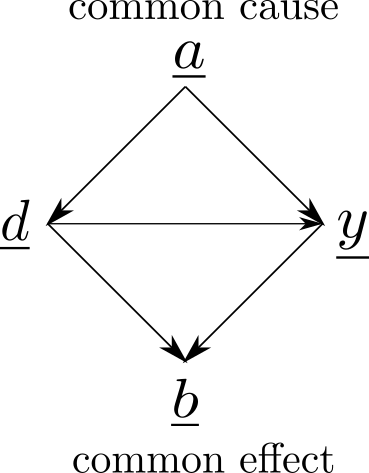
\includegraphics[width=1in]
{sb-removal/common-cause-effect.png}
\caption{Common Cause 
and Effect for 
nodes $\rvd,\rvy$.} 
\label{fig-common-cause-effect}
\end{figure}

Note
that in Potential
Outcomes (PO) theory
 (see Chapter \ref{ch-pot-out}),
root nodes such
as $\rva$ in
Fig.\ref{fig-common-cause-effect}
are called {\bf common cause
 (confounder, fork) nodes
for nodes $\rvd, \rvy$}.
Furthermore, leaf nodes such as 
$\rvb$ in
Fig.\ref{fig-common-cause-effect} are 
called 
{\bf common effect
(selection bias (SB), collider) nodes
for nodes $\rvd, \rvy$}.
Hence, in PO theory,
SB is indicated
by
a leaf node,
opposite to 
what we do in this chapter.

Note that 
{\bf Simpson's paradox} (see Chapter
\ref{ch-simpson}) arises from an indirect effect
caused by \ul{not conditioning} 
on a confounder,
whereas 
{\bf Berkson's paradox}
(see Chapter \ref{ch-berkson})
arises from an indirect effect
caused by \ul{conditioning}
on a collider.



\section{Removing SB from 
passive query $P(y|x)$}

The {\bf  passive query} $P(y|x, \rvs=1)$
is {\bf SB-recoverable}
if it is independent of $\rvs$
for some bnet $G$.







\begin{enumerate}
\item {\bf No SB.}
{\bf Query $P(y|x)$ is
SB-recoverable}
with $\rvA= \emptyset$; SB can be removed
by conditioning on $\rvx$.

If $\rvy\perp\rvs|\rvx$, then
\beq
P(y|x, \rvs=1)=P(y|x)
\;.
\eeq
For example,
$\rvy\perp\rvs|\rvx$ in the following bnet:

\beq
\begin{array}{c}
\xymatrix{
\rvs\ar[d]
\\
*++[o][F*:yellow]{\rvx}\ar[r]&\rvy
}
\\
\rvy\perp\rvs|\rvx
\end{array}
\eeq



\item {\bf Query $P(y|x)$ is
SB-recoverable}
via $\rvxi$; SB can be removed
by conditioning on $\rvx$
and $\rvxi$.
Here $\rvxi$
is a nonempty
subset of $\rvA$

\begin{claim}\label{cl-sb-recov}
There exists $\rvxi\subset \rvA$
 such that
 $\rvy\perp\rvs|(\rvx,\rvxi)$
and $\rvxi\perp\rvs|\rvx$
iff
\beq
P(y|x, \rvs=1)
=
\sum_\xi 
\underbrace{P(y|x, \xi, \rvs=1)}_
{P(y|x,\xi)}
\underbrace{P(\xi|x, \rvs=1)}_{P(\xi|x)}
=P(y|x)
\eeq

\beq
\xymatrix{
\rvs=1\ar[rd]
\\
x\ar[r]
&y
}
\xymatrix{\\=}
\xymatrix{
&\sum \xi\ar[d]
\\
x\ar[r]\ar[ru]
&y}
\xymatrix{
\\=}
\xymatrix{\\
x\ar[r]&y}
\eeq
\end{claim}
\proof

The $\Rightarrow$ part of this 
claim is obvious. For a proof
of the $\Leftarrow$ part, see
 Ref.\cite{bare-sb-removal}.
\qed

The simplest example
of a bnet to which
Claim \ref{cl-sb-recov}
applies is this:

\beq
\xymatrix{
\rvs\ar[d]
&{\rvxi}\ar[d]
\\
{\rvx}\ar[r]
\ar[ru]
&\rvy
}
\eeq

As a second example
of Claim \ref{cl-sb-recov},
consider the following bnet:
\beq
\xymatrix{
\rvs\ar[d]\ar@/^1pc/[rr]
&{\rvz}\ar[d]\ar[r]
&{\rvw}
\\
{\rvx}\ar[r]
\ar[ru]
&\rvy
}
\eeq

$\rvy\perp\rvs|(\rvx,\rvxi)$
and $\rvxi\perp\rvs|\rvx$
with $\rvxi=\rvz$
for this bnet:

\beq
\begin{array}{cc}
\xymatrix{
\rvs\ar[d]\ar@/^1pc/[rr]
&*++[o][F*:yellow]{\rvz}\ar[d]\ar[r]
&{\rvw}
&
\\
*++[o][F*:yellow]{\rvx}\ar[r]
\ar[ru]
&\rvy
}
&
\xymatrix{
\rvs\ar[d]\ar@/^1pc/[rr]
&{\rvz}\ar[d]\ar[r]
&{\rvw}
&
\\
*++[o][F*:yellow]{\rvx}\ar[r]
\ar[ru]
&\rvy
}
\\
(a)\quad 
\rvy\perp\rvs|(\rvx, \rvz)
&(b)\quad
\rvz\perp\rvs|\rvx
\end{array}
\label{eq-x-z-w-recov}
\eeq
Therefore

\beqa
P(y|x, \rvs=1)
&=&
\xymatrix{
&\sum {z}\ar[d]\ar[r]
&\sum{w}
&
\\
{x}\ar[r]
\ar[ru]
&y
}
\\
\eeqa

\item {\bf Query $P(y|x)$ is not
SB-recoverable}; SB cannot be removed.

\beq
\xymatrix{
\rvs\ar[d]\ar[dr]
\\
\rvx\ar[r]&\rvy
}
\quad\quad
\xymatrix{
\rvs\ar[dr]
\\
\rvx\ar[r]&\rvy
}
\quad\quad
\xymatrix{
\rvs\ar[r]\ar[d]
&\rvz\ar[dl]
\\
\rvx\ar[r]
&\rvy\ar[u]
}
\eeq


\end{enumerate}

\section{Removing SB from active query 
$P(y|{\cal D}x)$}

The {\bf active
query (i.e., do query)}
$P(y|\cald\rvx=x, \rvs=1)$
is 
\begin{enumerate}[(a)]
\item {\bf SB-recoverable}
if it equals $P(y|\cald\rvx=x)$
for some 
bnet $G$,
\item
{\bf do-identifiable}
if it equals
$P(y|x, \rvs=1)$ 
for some bnet $G$,
\item
both
{\bf SB-recoverable
and do-identifiable}
if it equals 
$P(y|x)$
for the same bnet $G$.
\end{enumerate}

Examples
\begin{itemize}
\item

\beq
\xymatrix{
\rvs\ar[r]
&\rvxi\ar[d]
\\
\rvx\ar[r]\ar[ru]
&\rvy}
\quad
\begin{array}{l}
\text{SB-recoverable: NO}
\\
\text{do-identifiable: YES}
\end{array}
\label{eq-sb-removal-ex-1}
\eeq
For bnet Eq.(\ref{eq-sb-removal-ex-1}),
$P(y|\cald\rvx=x, \rvs=1)$
is do-identifiable
because there are no unobserved nodes.
It's not SB-recoverable because
to block information
from flowing from $\rvy$ to $\rvs$,
one must condition on $\rvxi$.
But if one conditions on $\rvxi$,
then  info flows from $\rvx$ to $\rvs$,
which is forbidden by Claim
\ref{cl-sb-recov}.
\item

\beq
\xymatrix{
\rvs\ar[d]
&*++[F-o]{\rvxi}\ar[d]\ar[ld]
\\
\rvx\ar[r]
&\rvy
}\quad
\begin{array}{l}
\text{SB-recoverable: YES}
\\
\text{do-identifiable: NO}
\end{array}
\label{eq-sb-removal-ex-2}
\eeq
\end{itemize}


Let

$V=$ set of nodes in graph

$V^{<\rvx}=$ non-descendants 
of $\rvx$ (excluding $\rvx$)

$V^{>\rvx}=$ descendants
of $\rvx$ (excluding $\rvx$)

$\rvz^{<\rvx} = \rvz\cap V^{<\rvx}$

$\rvz^{>\rvx} = \rvz\cap V^{>\rvx}$


Suppose $\rvz \cup\{\rvx,\rvy\} \subset E$
and $\rvz\subset \rvA$.
We say $\rvz$ satisfies the {\bf 
selection bias (SB) 
backdoor criterion} 
with respect to $(\rvx, \rvy)$
if

\begin{enumerate}
\item all backdoor
paths from $\rvx$ to
$\rvy$ are blocked by conditioning on $\rvz^{<\rvx}$
\item $\rvz^{>\rvx} \perp \rvy | (\rvx,\rvz^{<\rvx})$
\item $\rvy\perp\rvs|(\rvx,\rvz)$
\end{enumerate}

 \begin{claim}(SB Backdoor
 Adjustment Formula)

If $\rvz$ satisfies the SB backdoor
criterion relative to $(\rvx, \rvy)$,
then

\beq
P(y|\cald\rvx=x, \rvs=1)
=
\sum_z P(y|x,z)P(z)=P(y|x)
\eeq

\beq
\xymatrix{
\rvs=1
\ar[rd]
\\
\cald\rvx=x\ar[r]
&y
}
\xymatrix{\\=}
\xymatrix{
&\sum z \ar[d]
\\
x\ar[r]
&y}
\\
\xymatrix{\\=}
\xymatrix{
\\
x\ar[r]&y
}
\eeq

\end{claim}
\proof

If
$z$
satisfies the
SB backdoor
criterion
relative
to
$(\rvx, \rvy)$,
then
$\rvx, \rvy, \rvz$
might
have the following 
structure.


\beq
\xymatrix{
\rvs\ar[d]\ar[r]\ar@/^1pc/[rr]
&\rvz^{<\rvx}\ar[ld]\ar[d]\ar[r]
&\rvz^{>\rvx}
\\
\rvx\ar[rru]\ar[r]
&\rvy
}
\label{eq-sb-bdoor-special}
\eeq

See Claim \ref{cl-decSBBackDoor}
for a proof of this claim
for the
special case Eq.(\ref{eq-sb-bdoor-special}).
\qed


